In this Alloy section we focused mainly on the two most critical point of S\&C: the opening and closing of an internship position and the application by a student to an open position.
At the end there are also some screenshot from the Alloy analyzer that proved our predicates to be consistent or say that assertion may be valid since no counterexample were found (which is equivalent to say that the assertions made were fine since Alloy does bounded verification). 
In order to improve the readability of the Alloy part we decided to divide the code into different sections, namely Signatures, Internship Positions, Applications and Feedback and Universities.
\begin{verbatim}
--------------------------------------------------------------------------------
Signatures:
--------------------------------------------------------------------------------
enum ApplicationStatus {Accepted, Rejected, Pending, ToBeAssessed, Confirmed, Refused}

enum InternshipStatus {Ongoing, Finished}

enum InternshipPositionStatus { Open, Closed }


abstract sig Feedback{
    rating: Int,
    review: String,
    internship: one Internship
}

abstract sig User {
    email:  String,
    password:  String,
}

sig Student extends User {
    username: String,
    var applications: set Application,
    var internships: set Internship,
    var university: one University
}

sig Company extends User {
    name: String
}

sig University {
    name: String,
    var internship: set Internship    
}

sig Internship {
    application: one Application,
    var status: InternshipStatus
} 

sig InternshipPosition {
    var applications: set Application,
    var status: InternshipPositionStatus
}

sig Application {
    company: one Company,
    internshipPosition: one InternshipPosition,
    student: one Student,
    var status: ApplicationStatus,
}

sig FeedbackByStudent extends Feedback {
    giver: one Student
}

sig FeedbackByCompany extends Feedback{
    giver: one Company
}
--------------------------------------------------------------------------------
Internship Positions
--------------------------------------------------------------------------------
// All internship positions are open at the beginning
fact DefaultOpenInternshipPosition {
    all i: InternshipPosition | i.status = Open
}



// Closed internship positions will not reopen
fact InternshipPositionClosedWontReopen {
	all i: InternshipPosition | 
		always (i.status = Closed implies
				 after always i.status = Closed)
}

// If an internship position is open, it will eventually be closed
fact NotAlwaysOpenInternshipPosition {
    all i: InternshipPosition | 
        always ( i.status = Open
                implies 
                    eventually i.status = Closed )
}
// If an internship position is open it has been open since the beginning
fact NowOpenPreviouslyOpenInternshipPosition {
    all i: InternshipPosition | 
        always ( i.status = Open
                    implies 
                        historically i.status = Open )
}


// If an internship position is closed now it has been closed in an instant in the past
fact IfClosedDidClose {
all i: InternshipPosition |
    always (i.status = Closed
        implies 
            once close[i])
}

// If I applied to an internship position it must have been open in the past
assert OnlyApplyToOpenInternshipPosition { 
    all a: Application | 
        always (once a.internshipPosition.status = Open)
        
}

check OnlyApplyToOpenInternshipPosition for 20 steps


pred close[i: InternshipPosition] {
    i.status = Open
    i.status' = Closed
}

run close for 15 but 4 InternshipPosition, 2 Company, 2 Student, 2 Application, 2 University, 4 steps


pred showThatInternshipCloses{
InternshipPosition.status = Open
after eventually Closed in InternshipPosition.status
}

run showThatInternshipCloses
\end{verbatim}
The results of the instructions above:
\begin{figure}[h!]
    \centering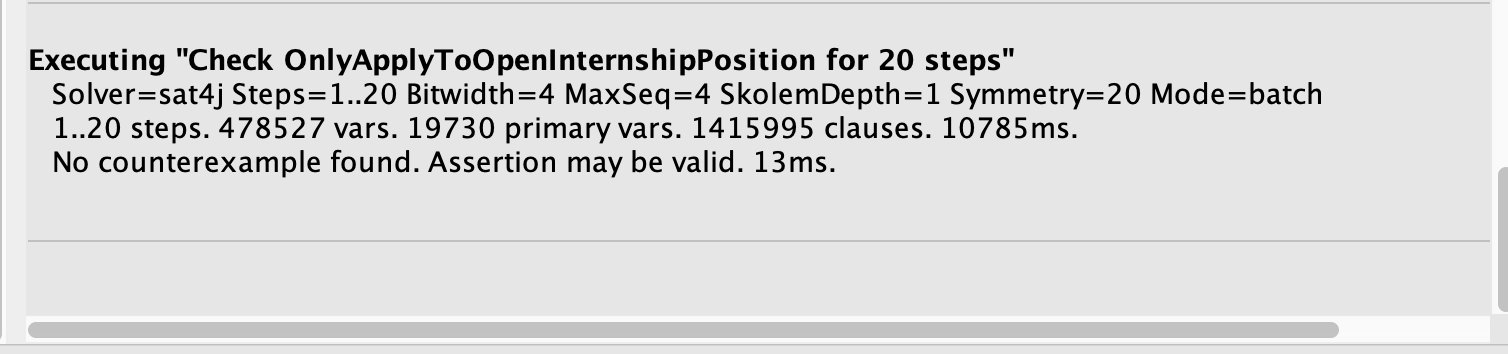
\includegraphics[width=0.5\textwidth]{RASD/Images/Alloy/checkOnlyApplyToOpenInternshipPosition.png}
    \label{fig:checkOnlyApplyToOpenInternshipPosition}
\end{figure}
\begin{figure}[h!]
    \centering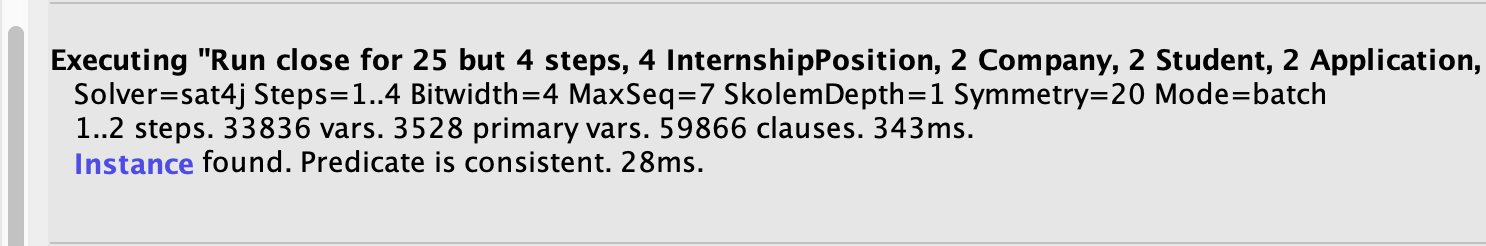
\includegraphics[width=0.5\textwidth]{RASD/Images/Alloy/predclose.png}
    \label{fig:predclose}
\end{figure}
\begin{figure}[h!]
    \centering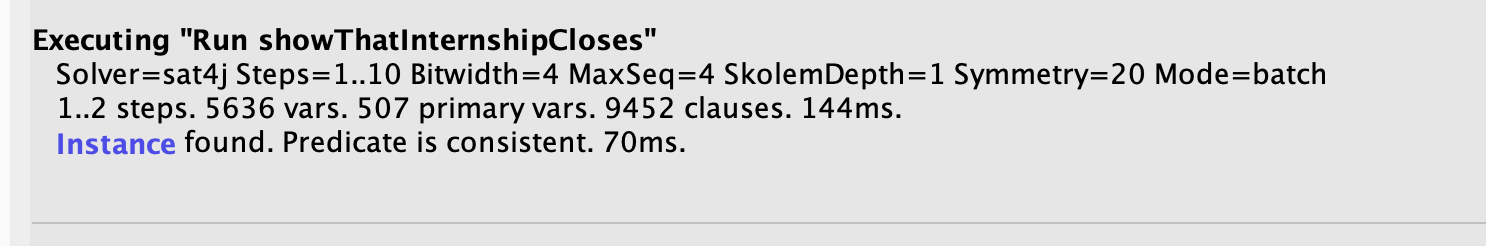
\includegraphics[width=0.5\textwidth]{RASD/Images/Alloy/predshowThatInternshipCloses.png}
    \label{fig:predshowThatInternshipCloses}
\end{figure}



\begin{verbatim}
--------------------------------------------------------------------------------
Applications
--------------------------------------------------------------------------------

// All applications are done to open positions
fact ApplicationsOnlyForOpenPositions {
    all a: Application | a.internshipPosition.status = Open
}

// All applications are pending at the beginning
fact DefaultPendingApplication {
    all a: Application | a.status = Pending
}

// If an application is pending, it will eventually be either rejected or confirmed or refused
fact EventualStatusOfPendingApplication {
    all a: Application | 
        always ( a.status = Pending
                implies 
                    eventually a.status = Rejected or 
                    a.status = Confirmed or a.status = Refused )
}
// If an application is pending, it will eventually be either rejected or confirmed or refused

fact EventuallyRejectedAcceptedToBeAssessedApplication {
    all a: Application | 
        always ( a.status = ToBeAssessed
                implies 
                    eventually a.status = Rejected or 
                    a.status = Confirmed or a.status = Refused )
}
// Pending applications are referred only to open internship positions
assert PendingApplicationReferToOpenPositions {
    all a: Application | 
        a.status = Pending implies a.internshipPosition.status = Open
}

// Pending applications are referred only to open internship positions
assert AcceptedApplicationReferToOpenPositions {
    all a: Application | 
        a.status = Accepted implies a.internshipPosition.status = Open
}

// Applications which request further assessment are referred only to open internship positions
assert TobeAssessedApplicationReferToOpenPositions {
    all a: Application | 
        a.status = ToBeAssessed implies a.internshipPosition.status = Open
}
\end{verbatim}
The results of the instructions above:
\begin{figure}[h!]
    \centering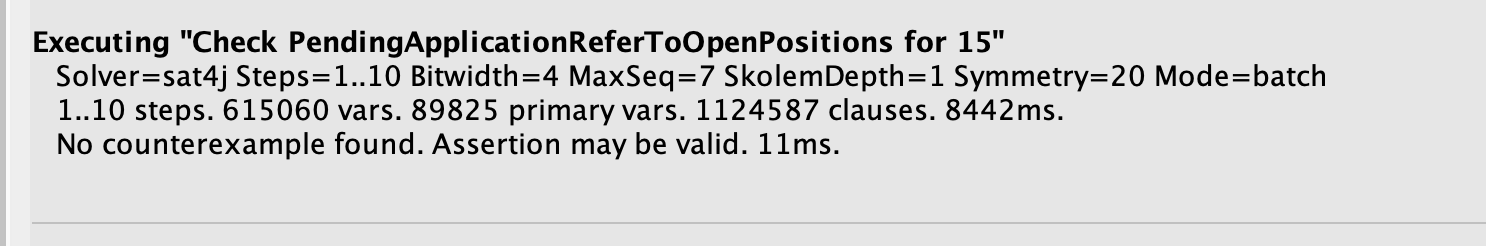
\includegraphics[width=0.5\textwidth]{RASD/Images/Alloy/checkPendingApplicationsReferToOpenPositions.png}
    \label{fig:checkPendingApplicationsReferToOpenPositions}
\end{figure}
\begin{figure}[h!]
    \centering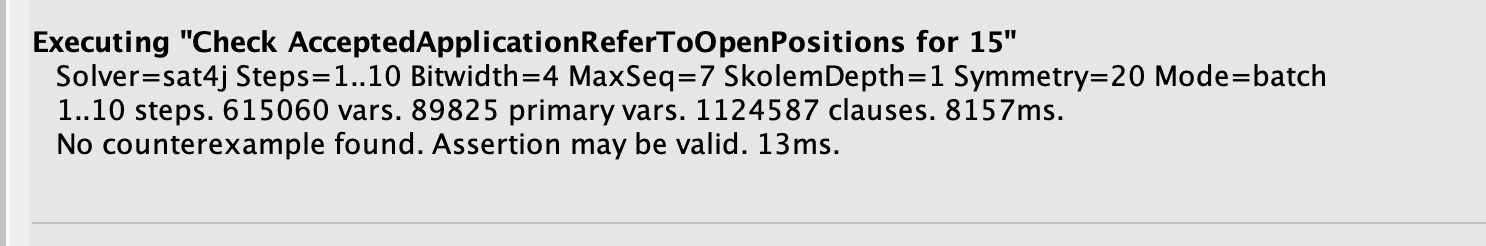
\includegraphics[width=0.5\textwidth]{RASD/Images/Alloy/checkAcceptedApplicationReferToOpenPositions.png}
    \label{fig:checkAcceptedApplicationReferToOpenPositions}
\end{figure}
\begin{figure}[h!]
    \centering\includegraphics[width=0.5\textwidth]{RASD/Images/Alloy/checkTobeAssessedApplicationReferToOpenPositions.png}
    \label{fig:TobeAssessedApplicationReferToOpenPositions}
\end{figure}


\begin{verbatim}

--------------------------------------------------------------------------------
Feedback and Universities
--------------------------------------------------------------------------------

// All feedbacks given by student are given after an internship is finished
assert FeedbackStudentGivenOnFinishedInternship {
    all f: FeedbackByStudent | f.internship.status = Finished
}
// All feedbacks given by copanies are given after an internship is finished
assert FeedbackCompanyGivenOnFinishedInternship {
    all f: FeedbackByCompany| f.internship.status = Finished
}
// A student can only give feedback for an internship he has taken
fact StudentFeedbackOnlyTheirInternship {
    all f: FeedbackByStudent | 
        f.giver in f.internship.application.student
}
// A company can only give feedback for an internship he has offered
fact CompanyFeedbackOnlyTheirInternship {
    all f: FeedbackByCompany | 
        f.giver in f.internship.application.company
}

fact UniversityMonitorsItsStudentsInternship {
    all u: University, i: Internship | 
        i in u.internship implies i.application.student.university = u
}

check FeedbackCompanyGivenOnFinishedInternship for 10

\end{verbatim}

The results of the instructions above:

\begin{figure}[h!]
    \centering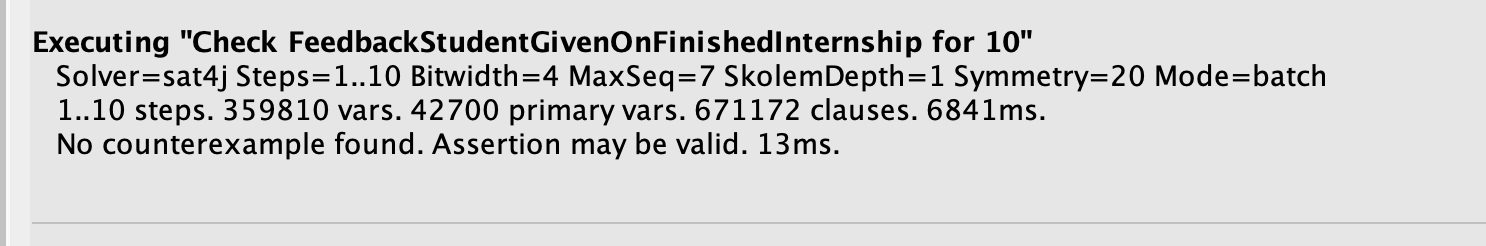
\includegraphics[width=0.5\textwidth]{RASD/Images/Alloy/checkFeedbackStudentGivenOnFinishedInternship.png}
    \label{fig:checkFeedbackStudentGivenOnFinishedInternship}
\end{figure}
\begin{figure}[h!]
    \centering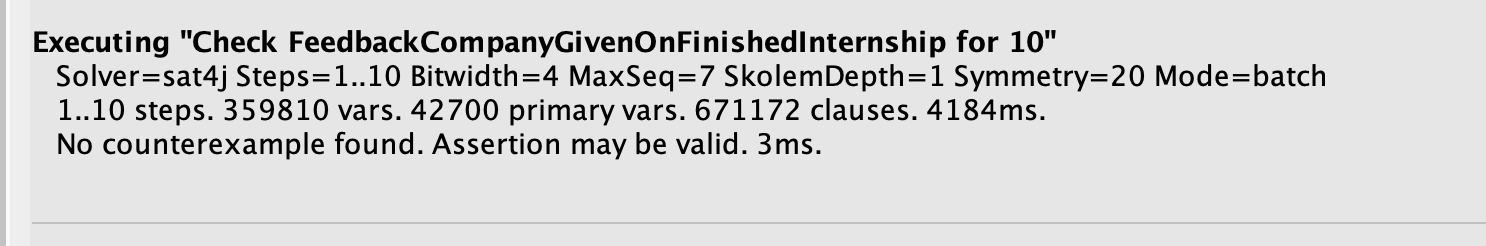
\includegraphics[width=0.5\textwidth]{RASD/Images/Alloy/checkFeedbackCompanyGivenOnFinishedInternship.png}
    \label{fig:checkFeedbackCompanyGivenOnFinishedInternship}
\end{figure}